\chapter{Results}
\section{Important Quantities from Our Model}
As shown in the previous chapter, our model describes the change in allele frequencies over time and space. Evolutionary forces act to shape the distribution of alleles across our simulated geographic habitat. There are two immediate questions that we will utilize our model to answer:

\begin{enumerate}
    \item How much of the allele do we expect to observe?
    \item Where can we expect to find the allele?
\end{enumerate}


For a more intuitive understanding of what each of these questions represent, let us examine the raw simulation output from our model. We simulate a single genetic locus and record the frequency of the minor, or \textit{focal} allele $f(a)$ after thousands of simulated generations. Allele frequencies vary across geographic position, but tend to be higher in some neighboring demes. This represents the localization of rare alleles observed in natural populations. \cite{1000_genomes} \cite{geerlings_2018} \cite{novembre_marcus_2017} 


\begin{figure}[h]
    \centering
    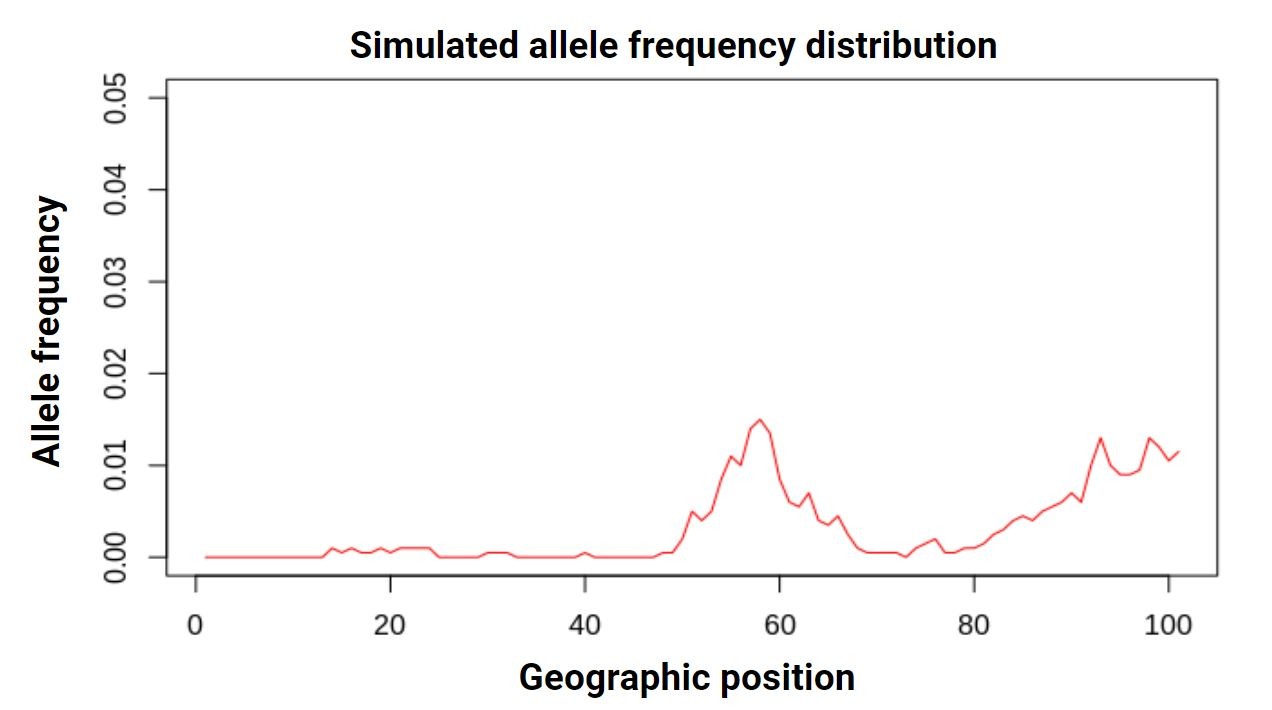
\includegraphics[scale=0.4]{img/geographic_distribution.JPG}
    \caption{The geographic distribution of the focal allele in a single simulation with a single set of evolutionary parameters ($\mu,s,m,N$). We allow for thousands of generations of time to pass to allow our simulation to approach equilibrium.}
    \label{fig:geog_sim}
\end{figure}


We observe a peak in the simulated example (Figure: \ref{fig:geog_sim}) that illustrates the geographic range of the allele. New alleles come into existence at one particular location. Some of these will reach higher frequencies in the population and some will spread farther beyond their initial position. The height of these peaks tells us how much of the allele we can expect to observe, and the width of these peaks tells us where we can expect to observe it. It is clear that alleles that reach, on average, higher frequencies will be easier to observe. We will calculate the average allele frequency and the geographic range of an allele to answer our initial questions.



\subsection{The average allele frequency}

\begin{figure}[h]
    \centering
    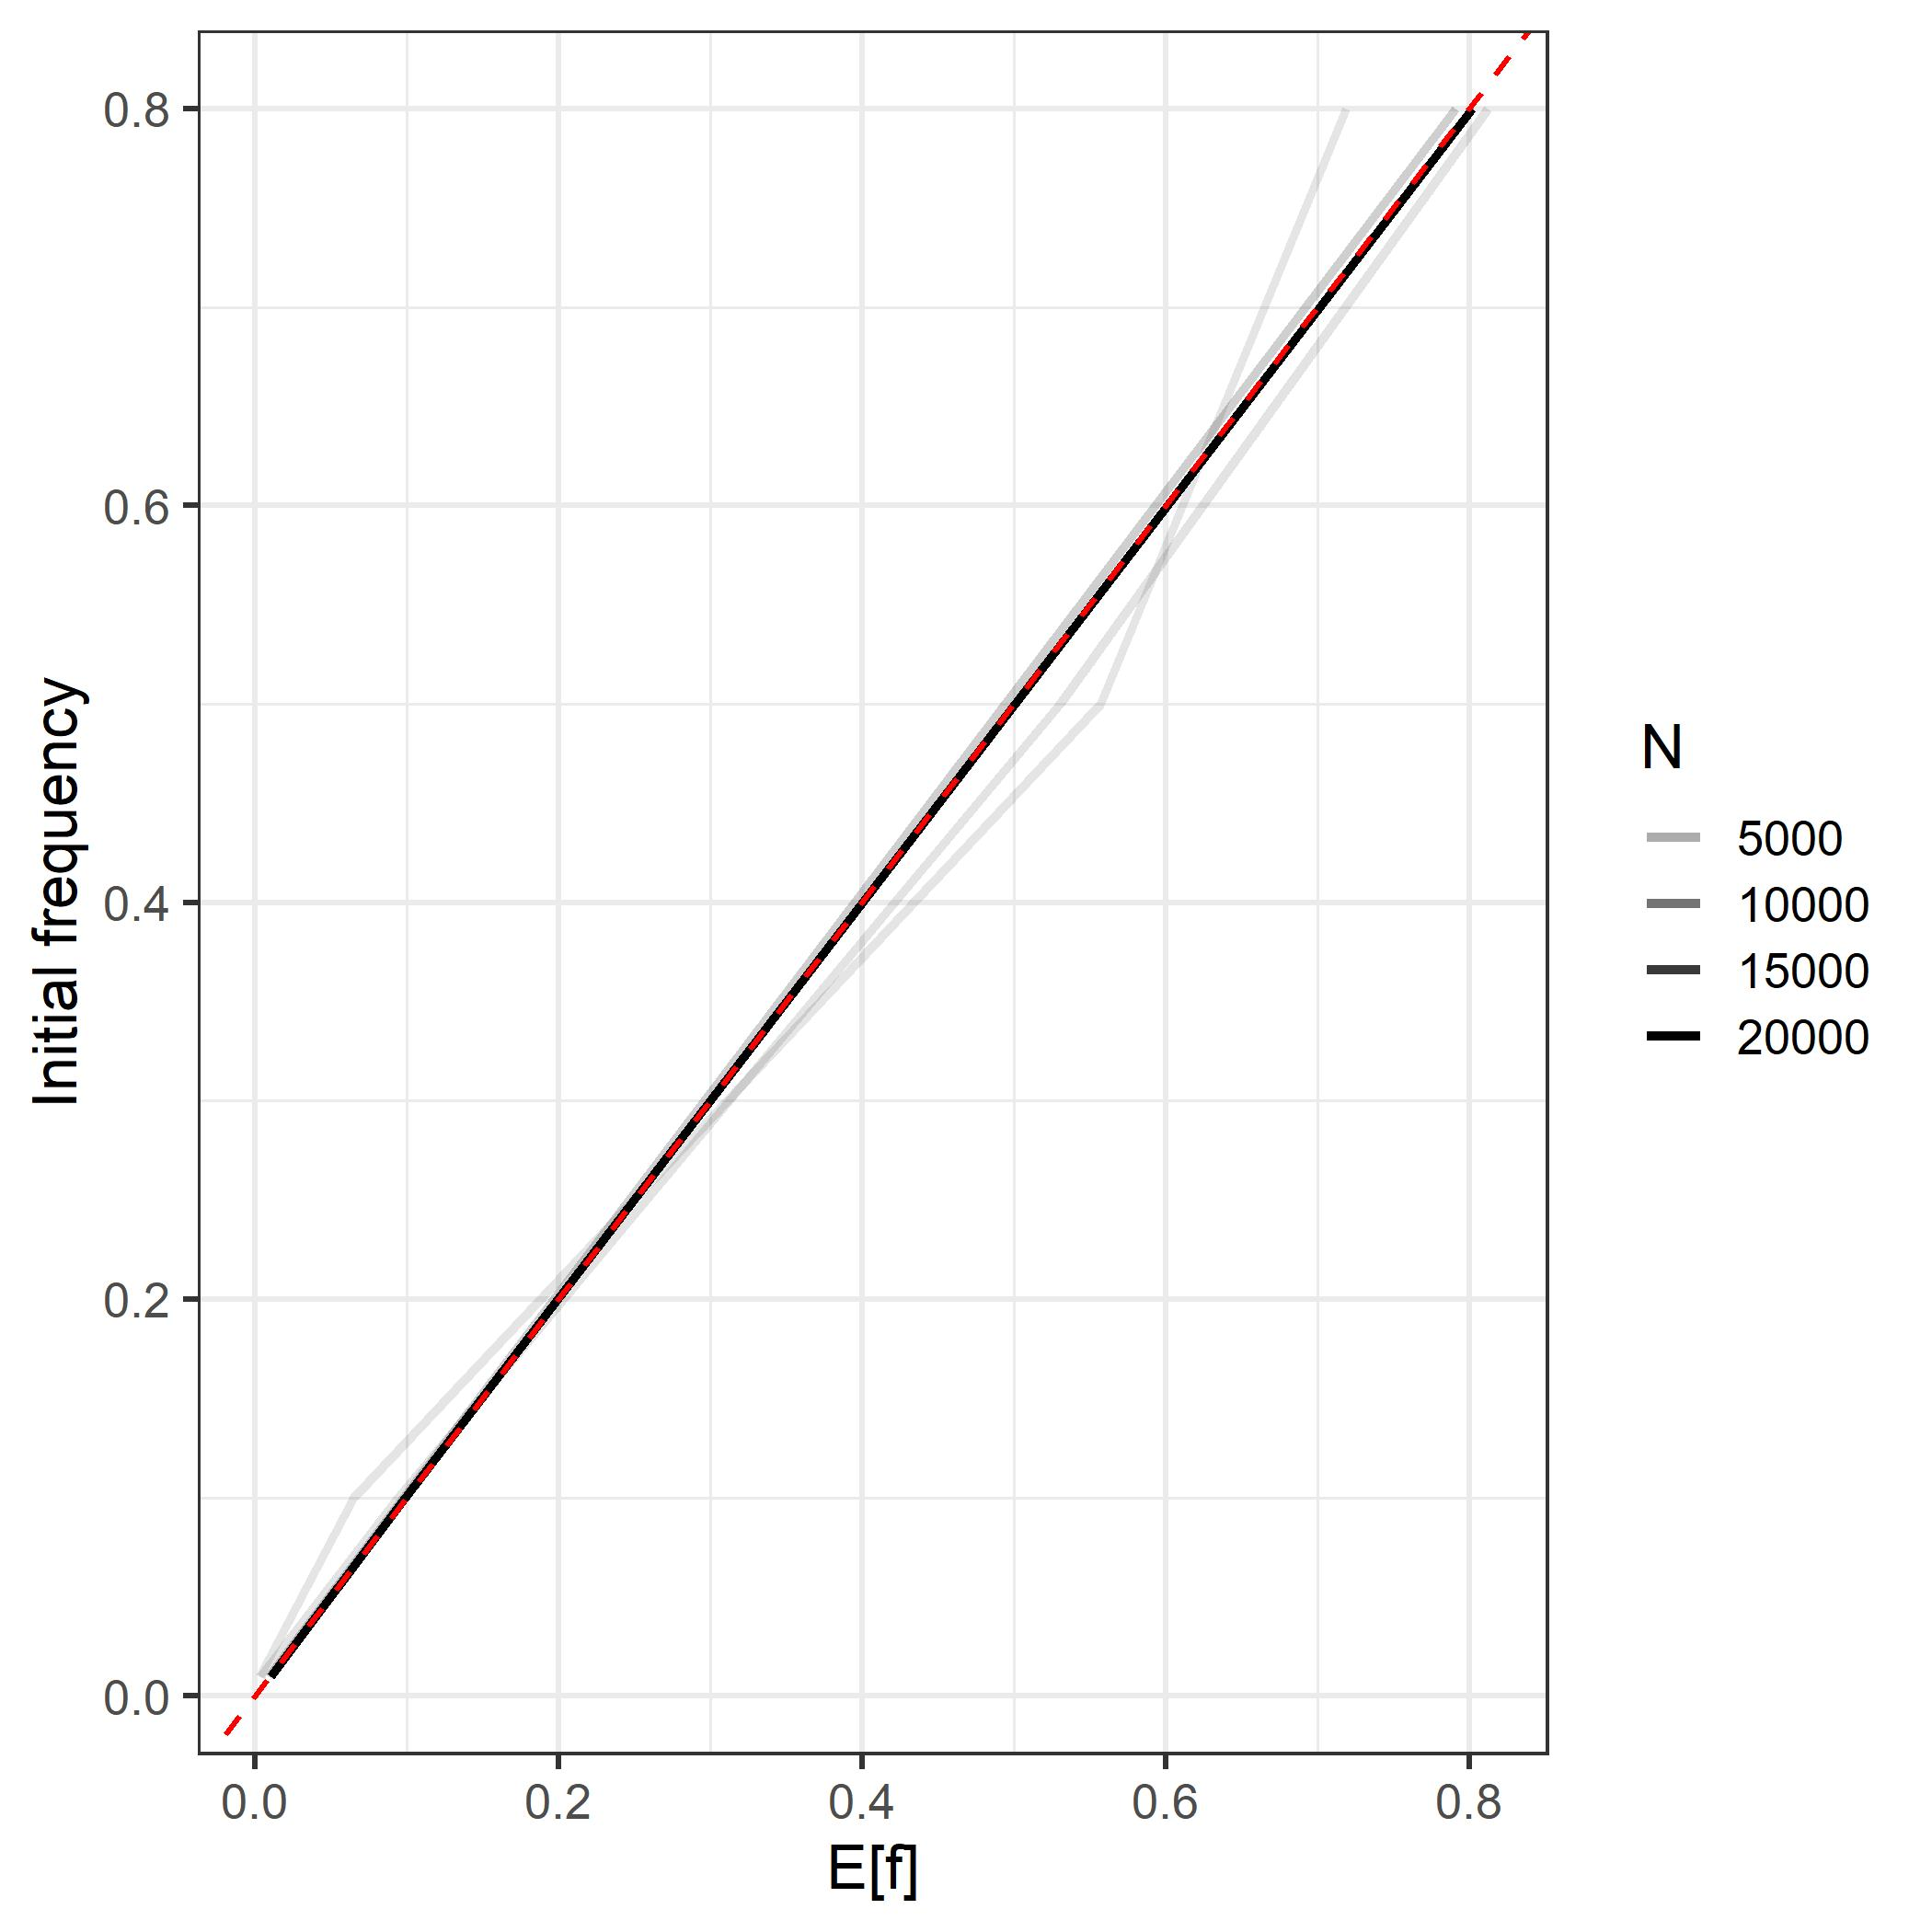
\includegraphics[scale=0.5]{img/mean_f.jpg}
    \caption{This figure confirms the neutral Wright-Fisher model average frequency. As predicted, $E[f] = f_0$. Simulations run at varying population sizes validate this prediction. The dashed, red line has y-intercept $0$ and slope $1$.}
    \label{fig:neutral_wf}
\end{figure}
 

\subsection{The geographic range of the allele}


\section{Computing the Expected Site Frequency Spectrum}

\section{Measuring Missing Heritability}